\subsection{Inheritance}
\begin{frame}[t]{Inheritance}
\begin{columns}[T, onlytextwidth]
\column{0.5\textwidth}
L1, \Venus\ (16 \Aquarius), was VOC, separating from \Square\  \Jupiter\ (14 \Taurus), L8 (the deceased person's wealth) by reception
\begin{block}{}
\textsl{"Separation by reception is something foul and a horrible thing" [JH 35]}
\end{block}
\Moon\ (28 \Leo) VOC separating from \Opposition\ \Venus\ (16 \Aquarius) \\
\Moon\ first to leave her sign \Leo\ $\Rightarrow$ \Virgo \\
$\Rightarrow$ \Trine\ \Mars\ (6 \Taurus), neither planet receives the other, and \\
since \Mars\ is not L8 he signifies prohibition \\
\vspace{0.25cm}
\Venus\ moves from \Aquarius\ to \Pisces \\
$\Rightarrow$ \Sextile\ \Mars\ (6 \Taurus), neither planet receives the other \\
shows the same as the \Moon

\column{0.5\textwidth}
\begin{center}
{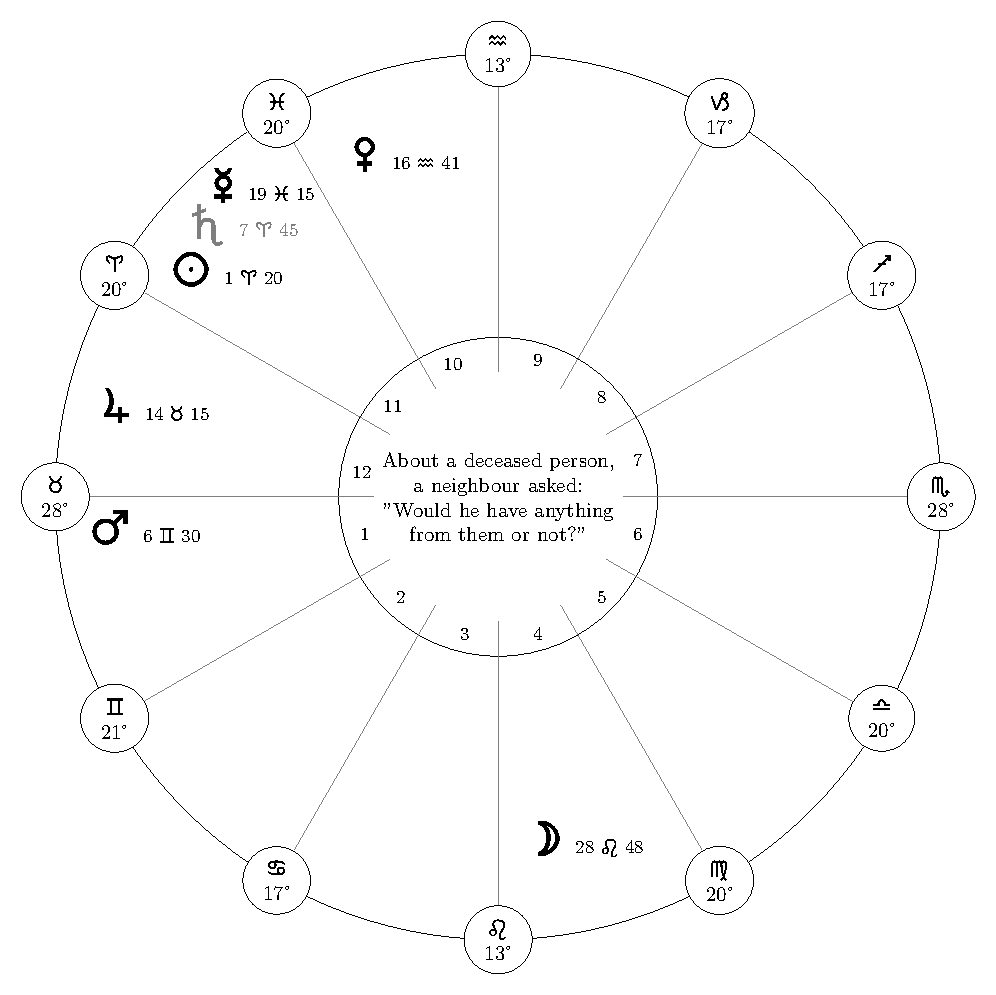
\includegraphics[width=0.9\textwidth]{charts/40-chart-inheritance}} \\
\small
House cusps are not original, Holden shows \Mercury\ as 20 \Pisces; Hand uses the degrees shown but puts \Mercury\ in the 10th
\end{center}
\end{columns}
\end{frame}